% 01 — Zadatak 1: QP, konveksnost, KKT, dualnost.

\section{Zadatak 1 --- kvadratično programiranje, KKT uvjeti i dualnost}
\label{sec:zad1}

\subsection{Formulacija problema}
\label{sec:zad1:formulacija}

Zadan je optimizacijski problem \cite[str.~1]{jokic_zadatak}
\begin{align}
  \min_{x}\quad & x_1^2 + 2x_2^2 - 0{,}3\,x_1x_2 + 2x_1 - 3x_2 \label{eq:z1cilj}\\
  \text{uz}\quad & a_{11}x_1 + a_{12}x_2 \le -10, \label{eq:z1g1}\\
                 & a_{21}x_1 + a_{22}x_2 \le 3, \label{eq:z1g2}
\end{align}
uz $a_{11}=-1$, $a_{12}=-1$, $a_{21}=1$, $a_{22}=-1$. Uvrštavanjem numeričkih
vrijednosti ograničenja postaju $x_1 + x_2 \ge 10$ i $x_1 - x_2 \le 3$.

Problem zapisujemo u standardnoj formi kvadratnog programa
$f(x) = \tfrac{1}{2}x^{\mathsf T}Hx + c^{\mathsf T}x$ uz $Ax \le b$
\cite[str.~34]{jokic_lpqp}, gdje je
\begin{equation}
  H = \begin{bmatrix} 2 & -0{,}3 \\ -0{,}3 & 4 \end{bmatrix}, \quad
  c = \begin{bmatrix} 2 \\ -3 \end{bmatrix}, \quad
  A = \begin{bmatrix} -1 & -1 \\ 1 & -1 \end{bmatrix}, \quad
  b = \begin{bmatrix} -10 \\ 3 \end{bmatrix}.
  \label{eq:z1std}
\end{equation}
Faktor $\tfrac12$ je nužan: dijagonalni članovi $H$ su dvostruki koeficijenti
kvadratnih članova, a izvandijagonalni je polovica koeficijenta mješovitog člana.

\subsection{Analiza konveksnosti}
\label{sec:zad1:konveksnost}

Funkcija cilja je konveksna ako i samo ako je njezina Hesseova matrica pozitivno
semidefinitna \cite[str.~61]{jokic_konveksnost}. Ovdje je $\nabla^2 f(x) = H$,
konstantna, sa svojstvenim vrijednostima
\begin{equation}
  \lambda(H) = \{1{,}955969,\; 4{,}044031\},
\end{equation}
dakle obje strogo pozitivne. Do istog zaključka vodi i Sylvesterov kriterij:
vodeći glavni minori su $2 > 0$ i $\det H = 8 - 0{,}09 = 7{,}91 > 0$.

Matrica $H$ je stoga pozitivno definitna, pa je $f$ \emph{strogo} konveksna.
Ograničenja \eqref{eq:z1g1}--\eqref{eq:z1g2} su linearna, pa je dozvoljeni skup
presjek dvaju poluravnina --- konveksan poliedar. Riječ je dakle o konveksnom
optimizacijskom problemu, i to strogo konveksnom QP-u. Posljedice su bitne za
sve što slijedi: rješenje je jedinstveno ako postoji, svaki lokalni minimum je
ujedno i globalni, a KKT uvjeti su ne samo nužni nego i \emph{dovoljni}.

\subsection{KKT uvjeti optimalnosti i njihovo rješenje}
\label{sec:zad1:kkt}

Uz Lagrangeovu funkciju $L(x,\lambda) = f(x) + \lambda^{\mathsf T}(Ax-b)$,
KKT uvjeti \cite[str.~59]{jokic_kkt} glase
\begin{align}
  Hx + c + A^{\mathsf T}\lambda &= 0 && \text{(stacionarnost)}, \label{eq:kkt1}\\
  Ax - b &\le 0 && \text{(primarna dopustivost)}, \\
  \lambda &\ge 0 && \text{(dualna dopustivost)}, \\
  \lambda_i\,(A_ix - b_i) &= 0,\quad i=1,2 && \text{(komplementarnost)}. \label{eq:kkt4}
\end{align}

Uvjet komplementarnosti \eqref{eq:kkt4} znači da je svako ograničenje ili
aktivno ($A_ix = b_i$, uz $\lambda_i \ge 0$) ili neaktivno ($A_ix < b_i$, uz
$\lambda_i = 0$). Sustavan postupak je stoga proći kroz sve $2^m$ kombinacija
aktivnih skupova i potražiti onu koja zadovoljava \emph{sve} KKT uvjete. Uz
$m = 2$ ograničenja to su četiri slučaja. Za pretpostavljeni aktivni skup $S$
rješava se linearan sustav
\begin{equation}
  \begin{bmatrix} H & A_S^{\mathsf T} \\ A_S & 0 \end{bmatrix}
  \begin{bmatrix} x \\ \lambda_S \end{bmatrix}
  = \begin{bmatrix} -c \\ b_S \end{bmatrix},
  \label{eq:kktsys}
\end{equation}
a zatim se provjeravaju primarna dopustivost $Ax \le b$ i dualna dopustivost
$\lambda \ge 0$. Rezultati su u tablici~\ref{tab:z1cases}.

\begin{table}[htbp]
  \centering
  \caption{Nabrajanje aktivnih skupova. Točno jedan slučaj zadovoljava sve KKT uvjete.}
  \label{tab:z1cases}
  \begin{tabular}{lccl}
    \hline
    Aktivni skup & $x$ & $\lambda$ & Status \\
    \hline
    $\{\}$          & $(-0{,}8976,\; 0{,}6827)$ & $(0,\; 0)$ & odbačen: nedopustiv \\
    $\{g_1\}$       & $(5{,}7576,\; 4{,}2424)$  & $(12{,}2424,\; 0)$ & \textbf{zadovoljava sve} \\
    $\{g_2\}$       & $(2{,}2407,\; -0{,}7593)$ & $(0,\; -6{,}7093)$ & odbačen: nedopustiv \\
    $\{g_1, g_2\}$  & $(6{,}5000,\; 3{,}5000)$  & $(11{,}5000,\; -2{,}4500)$ & odbačen: $\lambda_2 < 0$ \\
    \hline
  \end{tabular}
\end{table}

Slučaj bez aktivnih ograničenja daje bezuvjetni minimum $-H^{-1}c$, koji je
nedopustiv jer je $x_1 + x_2 = -0{,}215 < 10$. Slučaj $\{g_2\}$ je također
nedopustiv, a slučaj s oba aktivna ograničenja daje negativan množitelj
$\lambda_2 = -2{,}45$, čime pada na dualnoj dopustivosti. Preostaje jedini
kandidat
\begin{equation}
  x^\star = \begin{bmatrix} 190/33 \\ 140/33 \end{bmatrix}
          = \begin{bmatrix} 5{,}757576 \\ 4{,}242424 \end{bmatrix}, \qquad
  \lambda_1^\star = \frac{404}{33} = 12{,}242424, \qquad \lambda_2^\star = 0 .
  \label{eq:z1sol}
\end{equation}

Za njega je $\lambda_1^\star > 0$, drugo ograničenje je neaktivno jer je
$x_1^\star - x_2^\star - 3 = -1{,}484848 < 0$, što je konzistentno s
$\lambda_2^\star = 0$ u \eqref{eq:kkt4}, a rezidual stacionarnosti iznosi
$\lVert Hx^\star + c + \lambda_1^\star A_1^{\mathsf T}\rVert \approx 1{,}8\cdot10^{-15}$.
Optimalna vrijednost je
\begin{equation}
  p^\star = f(x^\star) = \frac{2000}{33} = 60{,}606061 .
\end{equation}
Budući da je problem konveksan, KKT uvjeti su dovoljni, pa je $x^\star$ globalni
minimizator, a zbog stroge konveksnosti i jedini.

\subsection{Grafički prikaz dozvoljenog skupa i gradijenata}
\label{sec:zad1:graficki}

Slika~\ref{fig:z1} prikazuje dozvoljeni skup, nivo krivulje funkcije cilja te
gradijente u točki $x^\star$. Gradijenti su
\begin{equation}
  \nabla f(x^\star) = Hx^\star + c = \begin{bmatrix} 12{,}242424 \\ 12{,}242424 \end{bmatrix}, \qquad
  \nabla g_1(x^\star) = \begin{bmatrix} -1 \\ -1 \end{bmatrix}, \qquad
  \nabla g_2(x^\star) = \begin{bmatrix} 1 \\ -1 \end{bmatrix}.
\end{equation}
Gradijenti ograničenja su konstantni jer su ograničenja afina, pa ne ovise o
točki u kojoj se računaju.

Geometrijski sadržaj stacionarnosti vidi se izravno: $\nabla f(x^\star)$ i
$\nabla g_1(x^\star)$ su antiparalelni, jer je
$\nabla f(x^\star) = -\lambda_1^\star \nabla g_1(x^\star)$. Nivo krivulja kroz
$x^\star$ tangira pravac $x_1 + x_2 = 10$; da nije tako, pomak duž granice
smanjio bi cilj i točka ne bi bila optimalna. Gradijent cilja pokazuje iz
dozvoljenog skupa prema van, što je upravo uvjet da se cilj ne može dodatno
smanjiti bez izlaska iz dozvoljenog skupa.

\begin{figure}[htbp]
  \centering
  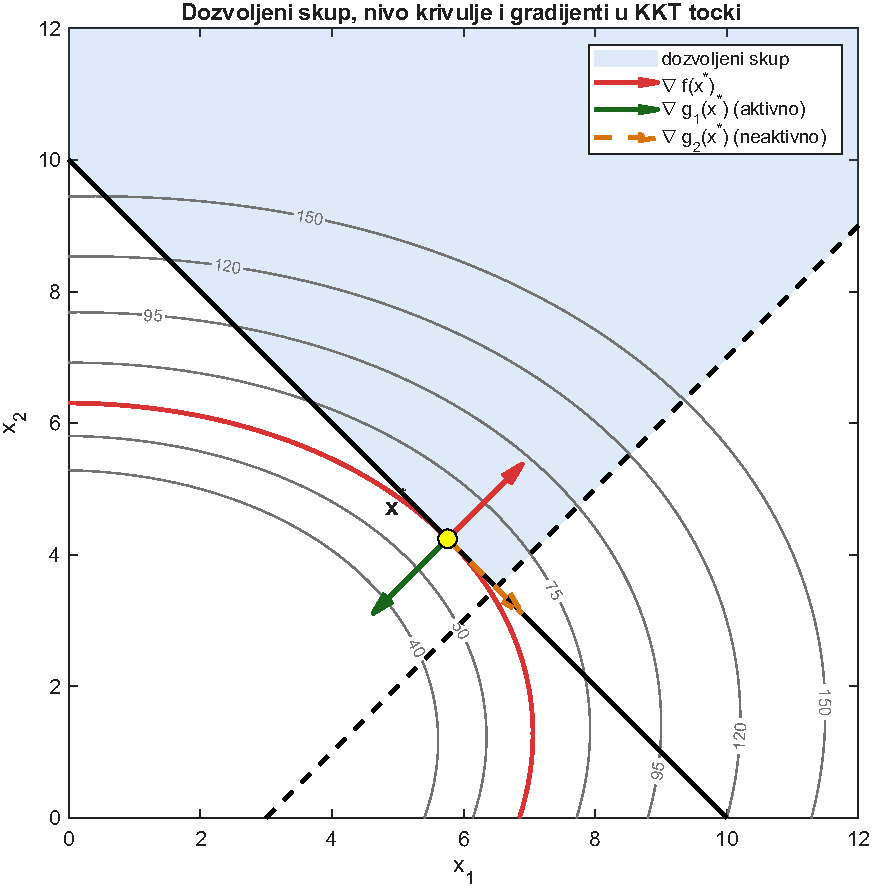
\includegraphics[width=0.78\textwidth]{figures/zad1_kkt.pdf}
  \caption{Dozvoljeni skup (plavo), nivo krivulje funkcije cilja, aktivno
  ograničenje (puna crta), neaktivno ograničenje (crtkano) te gradijenti
  funkcije cilja i obaju ograničenja u točki $x^\star$. Crvena krivulja je nivo
  krivulja $f(x) = p^\star$.}
  \label{fig:z1}
\end{figure}

\subsection{Numeričko rješenje u MATLAB-u}
\label{sec:zad1:matlab}

Problem je riješen dvama neovisnim putevima, funkcijom \texttt{quadprog} iz
Optimization Toolboxa i modeliranjem u YALMIP-u. Oba vraćaju
\begin{equation}
  x^\star = (5{,}757576,\; 4{,}242424)^{\mathsf T}, \qquad
  \lambda^\star = (12{,}242424,\; 0)^{\mathsf T},
\end{equation}
uz odstupanje od analitičkog rješenja \eqref{eq:z1sol} reda $10^{-11}$
(\texttt{quadprog}) odnosno $10^{-16}$ (YALMIP). Lagrangeovi množitelji koje
vraćaju solveri poklapaju se s onima izračunatima iz KKT sustava, što je i
očekivano: za konveksan QP množitelji su jedinstveni kad su gradijenti aktivnih
ograničenja linearno nezavisni, a ovdje je aktivno samo jedno ograničenje.

\subsection{Lagrangeov dualni problem}
\label{sec:zad1:dual}

Dualna funkcija je $g(\lambda) = \min_x L(x,\lambda)$. Kako je $H \succ 0$,
minimizacija po $x$ ima zatvorenu formu: iz $\nabla_x L = Hx + c + A^{\mathsf T}\lambda = 0$
slijedi $x = -H^{-1}(c + A^{\mathsf T}\lambda)$, pa je
\begin{equation}
  g(\lambda) = -\tfrac{1}{2}\,(c + A^{\mathsf T}\lambda)^{\mathsf T} H^{-1} (c + A^{\mathsf T}\lambda) - \lambda^{\mathsf T}b .
  \label{eq:dualfun}
\end{equation}
Dualni problem je $\max_{\lambda \ge 0} g(\lambda)$; to je konkavna maksimizacija,
dakle konveksan problem \cite[str.~24]{jokic_dualnost}.

Numeričko rješavanje \eqref{eq:dualfun} daje
\begin{equation}
  \lambda^\star = (12{,}242424,\; 0)^{\mathsf T}, \qquad d^\star = 60{,}606061 ,
\end{equation}
što se poklapa s množiteljima iz (b) i (d). Dualni jaz je
$p^\star - d^\star \approx 10^{-8}$, dakle numerički nula. Jaka dualnost je i
očekivana: problem je konveksan, a ograničenja su afina, pa je Slaterov uvjet
zadovoljen već postojanjem strogo dopustive točke \cite[str.~28]{jokic_dualnost}.

\subsection{Osjetljivost optimalne vrijednosti na perturbacije ograničenja}
\label{sec:zad1:osjetljivost}

Lagrangeovi množitelji imaju izravnu interpretaciju kao osjetljivost optimalne
vrijednosti na popuštanje ograničenja:
\begin{equation}
  \frac{\partial p^\star}{\partial b_i} = -\lambda_i^\star .
  \label{eq:sens}
\end{equation}
Uvrštavanjem rezultata \eqref{eq:z1sol}:
\begin{equation}
  \frac{\partial p^\star}{\partial b_1} = -12{,}242424, \qquad
  \frac{\partial p^\star}{\partial b_2} = 0 .
\end{equation}

Numerička provjera centralnom razlikom uz $\varepsilon = 10^{-6}$ daje
$-12{,}242424$ i $0{,}000000$, u skladu s \eqref{eq:sens}.

Tumačenje je sljedeće. Povećanje $b_1$ za $\Delta$ znači popuštanje aktivnog
ograničenja, pa optimalna vrijednost pada za približno $12{,}24\,\Delta$ --- to je
ograničenje koje stvarno „košta“. Ograničenje \eqref{eq:z1g2} je neaktivno, pa
njegova mala perturbacija ne mijenja rješenje: postoji rezerva od
$1{,}484848$ prije nego što ono postane aktivno, i tek za perturbacije veće od te
rezerve odnos \eqref{eq:sens} prestaje vrijediti. Relacija je lokalna i vrijedi
dok se skup aktivnih ograničenja ne promijeni.
